\subsection{Housing}
\label{sec:housing}

\textbf{Purpose}: \textit{Isolates} and \textit{insulates} growth environment from surroundings (heat, light, water vapour, air). Provides structural integrity and mounting points for other subsystems, and enables system extendability via repeated "unit cell" topology.

\textbf{Method}:
\begin{enumerate}
    \item \textit{Setup}:
    \begin{enumerate}
        \item Assemble frame and insert panels;
        \item Mount control module (w/ subsystems), connect inputs;
        \item Install tray mounts, insert trays (w/ subsystems);
    \end{enumerate}
    \item \textit{Testing}:
    \begin{itemize}
        \item Frame construction is rigid, level, and sturdy;
        \item Panels are insulating against temperature changes, and mitigate water vapour loss;
    \end{itemize}
    \item \textit{Process}:
    \begin{enumerate}
        \item Panels insulate against heat gain/loss, are opaque, and contain light and heat via reflection;
        \item Shell construction is tight, thus sealing against moisture;
        \item Internal vertical mounting channels for systems and horizontal plane "trays";
        \item Self-contained control module with all subsystem supplies, as well as automation systems;
        \item Solenoid lock to prevent unintended opening;
        \item \textbf{Housing Extension} (can be repeated):
        \begin{enumerate}
            \item Add a second housing;
            \item Remove dividing panel from both housings;
            \item Remove "shared" skeleton extrusions from second housing;
            \item Join the two housings to form one larger 2x1 housing;
            \item \textbf{Extension Modes} (may be combined in any way to suit application):
            \begin{itemize}
                \item \textit{Class 1} (no combined units, frame connection only): Leave the dividing panel, add a control module, and operate the two PeaPods \textbf{separately}.
                \item \textit{Class 2} (for 2-4 unit housing combinations): Operate the combined housing off \textbf{one} control module.
                \item \textit{Class 3} (for 5+ unit housing combinations): Add control modules to account for additional air volume, plant count, power requirement, etc. and operate in a \textbf{master-slaves topology}.
            \end{itemize}
        \end{enumerate}
    \end{enumerate}
    \item \textit{Shutdown}:
    \begin{enumerate}
        \item Dismount all systems, remove trays;
        \item Disassemble housing;
    \end{enumerate}
\end{enumerate}

\textbf{Features}:
\begin{itemize}
    \item \textit{Control Module}: Top-mounted self-contained module encapsulating all system inputs (incl. power, water, pH and nutrient solutions, network connection), subsystem supplies and controls (incl. power supply, all aeroponics (see \ref{sec:aeroponics}), thermoregulation control (see \ref{sec:airthermoregulation}), humidity control (see \ref{sec:humidification}, \ref{sec:dehumidification}), gas composition and exchange (see \ref{sec:gas})), and automation systems (see \ref{sec:automation}).
    \item \textit{Frame}: T-slotted aluminum extrusion framing with face-mounted brackets forms a cubic skeleton for rigidity/strength (high strength-to-weight aluminum) and easy component mounting and repositioning (standard mounting channels). These extrusions form the "edges" of the cubic housing. %Todo: cite extrusion
    \item \textit{Panels}: Graphite-enhanced expanded polystyrene (GPS) rigid foam insulation panels \cite{insulation} with reflective mylar internal lamination increase energy efficiency (GPS RSI of 0.0328$\frac{m^2 \cdot \degree C}{W}$ per mm of thickness, mylar enables light/heat reflection), as well as safety against cross-contamination and pathogens. Panels press-fit into the frame and form a "seal" for greater water vapour retention. %Todo: cite mylar
    \item \textit{Solenoid Lock}: Normally-open solenoid lock engages on-demand to prevent unintended contact with environment. Mitigates cross-contamination and maintains environment accuracy.
    \item \textit{Trays}: Horizontal plane subframes mounted to internal vertical extrusion channels for ease of leveling and repositioning. Trays slide in/out on mounting points. All connections are quick-connect for ease of tray removal (i.e. quick-disconnect tubing for grow tray, spring-loaded connectors for lighting power). Trays include:
    \begin{itemize}
        \item \textit{Grow Trays}: Support plants (via grow cups), aeroponic nozzles, aeroponics container, supply/recycling lines (see \ref{sec:aeroponics}), and side-view camera (see \ref{sec:automation}).
        \item \textit{Lighting Trays}: Support LED boards, driver board (see \ref{sec:lighting}), and top-down camera (see \ref{sec:automation}).
    \end{itemize}
\end{itemize}

\clearpage

\textbf{Figures}

\begin{figure}[h!]
    \centering
    \frame{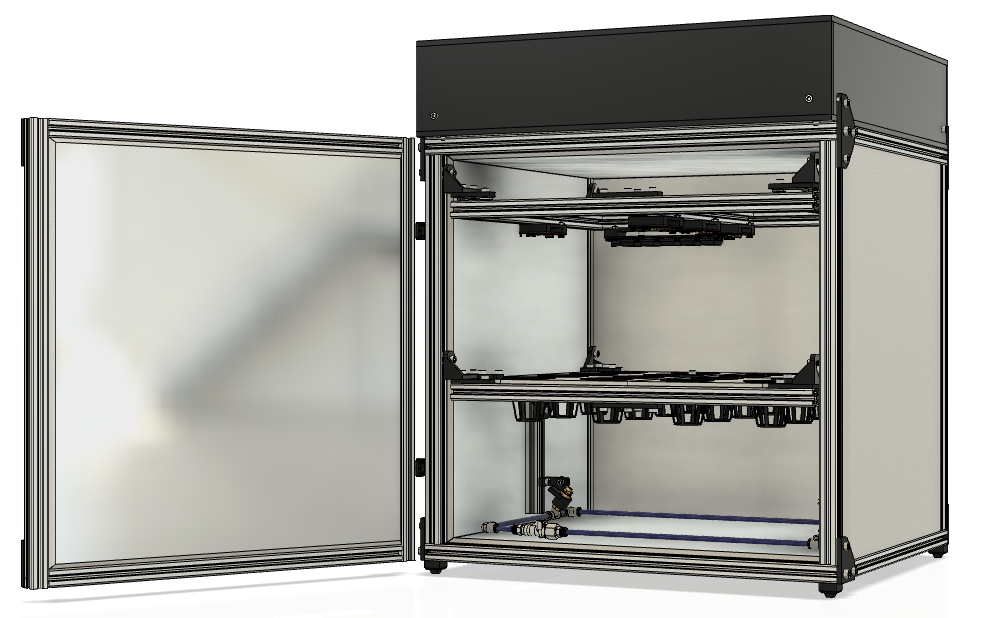
\includegraphics[width=\textwidth]{../assets/figures/housing_single.png}}
    \caption{Single-unit PeaPod, door open. Note the lighting tray (top) and grow tray (bottom), as well as the control module.}
    \label{fig:housing_single}
\end{figure}

\begin{figure}[h!]
    \centering
    \frame{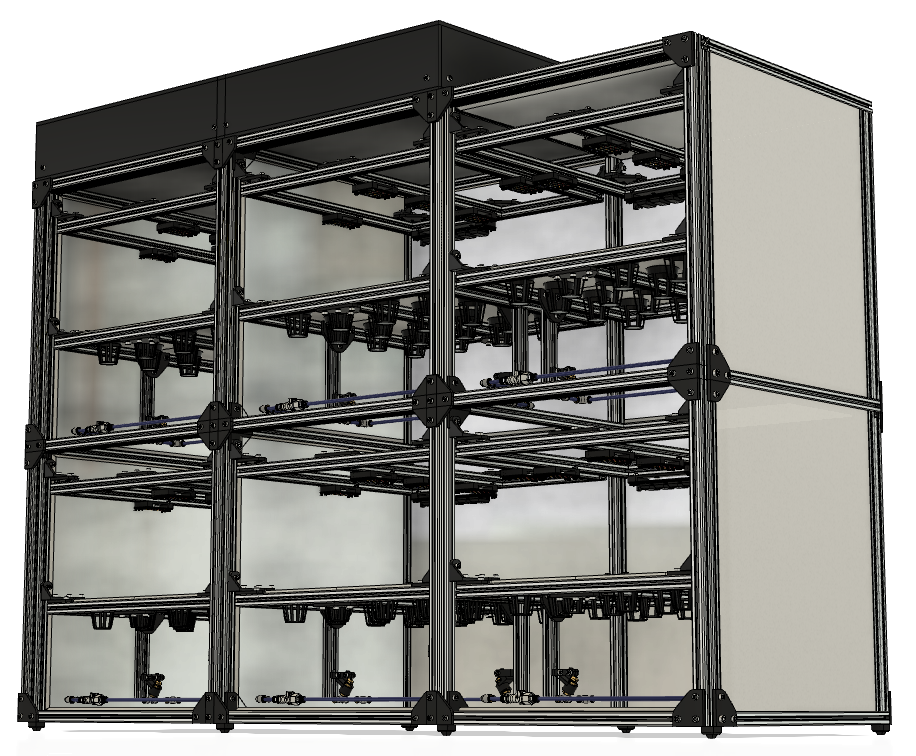
\includegraphics[width=\textwidth]{../assets/figures/housing_extended.png}}
    \caption{6-unit extended PeaPod, door panels removed, split into 2-unit (left) and 4-unit (right) Class 2 topologies, joined in a Class 1 topology.}
    \label{fig:housing_extended}
\end{figure}